\fig{fv:e1:rope}{绳冲量只调整沿绳分量，垂直分量可以保留}{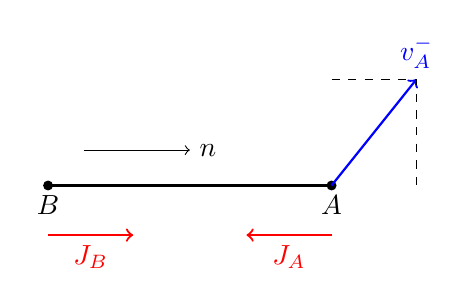
\begin{tikzpicture}[scale=.9]
\draw[thick](0,0)--(4,0);\fill(0,0)circle(2pt)node[below]{$B$};\fill(4,0)circle(2pt)node[below]{$A$};
\draw[->,blue,thick](4,0)--(5.2,1.5)node[above]{$\bm v_A^-$};\draw[dashed](4,1.5)--(5.2,1.5)--(5.2,0);
\draw[->,red,thick](4,-.7)--(2.8,-.7)node[midway,below]{$\bm J_A$};\draw[->,red,thick](0,-.7)--(1.2,-.7)node[midway,below]{$\bm J_B$};
\draw[->](.5,.5)--(2,.5)node[right]{$\bm n$};\end{tikzpicture}}
图\ref{fv:e1:rope}中两冲量等大反向，故总动量不变；各自又都沿绳，故不能改变垂直绳的速度分量。绷紧后的条件只是 $\bm v_A^+\cdot\bm n=\bm v_B^+\cdot\bm n$，并非两个速度矢量完全相同。先用这一投影条件解冲量，再检查冲量确为拉向对方，最后比较初末动能，便能同时区分守恒量、几何约束和非弹性耗散。
